\documentclass{IEEEtran}

\special{papersize=7.875in,10.75in}
\usepackage{amsmath}
\usepackage{amssymb}
\usepackage{mathptm}
\usepackage{url}
\usepackage{times}
\usepackage{graphicx,color}
\usepackage{CJKutf8}
\usepackage{multirow}
\usepackage{kotex}
\usepackage{gensymb}
%\usepackage{stfloats}


\setlength{\emergencystretch}{2em}
\setlength{\parindent}{0em}

\begin{document}

\title{Formation Eco-Driving for Heterogeneous Electric Vehicles}

\author{
Donkyu~Baek,~\IEEEmembership{Member,~IEEE,}  
Min Jae Jung,~\IEEEmembership{Student Member,~IEEE,}
Jaemin Kim,~\IEEEmembership{Student Member,~IEEE,}
and~Naehyuck~Chang,~\IEEEmembership{Fellow,~IEEE}

%\footnote{Corresponding author}, 
\thanks{
This work was supported by the National Research Foundation of Korea (NRF) grant funded by the Korea government (MSIP) (No.2015R1A2A1A09005694.) 

D. Baek is with the Control and Computer Engineering, Politecnico di Torino, Torino, Italy (e-mail: donkyu.baek@polito.it.)

M. Jung and N. Chang are with the School of Electrical Engineering, Korea Advanced Institute of Science and Technology, Daejeon, Republic of Korea (e-mail: minjae@cad4x.kaist.ac.kr; naehyuck@cad4x.kaist.ac.kr.)

J. Kim is with the Department of Computer Science and Engineering, Seoul National University, Republic of Korea (e-mail: jmkim@snu.ac.kr.)

Direct questions and comments about this article to Naehyuck Chang (naehyuck@cad4x.kaist.ac.kr.)}
%\thanks{Paper Number: ...}
%\thanks {Digital Object Identifier: }
}

\maketitle

\begin{abstract}
Formation driving is to accelerate and cruise multiple vehicles for less fuel consumption and a higher throughput. This paper introduces formation eco-driving for battery electric vehicles (BEV or all-electric vehicles powered solely by the battery.) We derive the least-energy cruising speed of the whole BEVs in the formation using V2V (vehicle to vehicle) communications exchanging the vehicle power models and calculating the most efficient allowable speed for each BEV in the formation. 
%We define the most efficient driving that achieves the least energy-delay product. The energy-delay product optimization allows us to consider both energy and throughput at the same time as a single metric. 
To address the problem more practically, we assume the formation is not necessarily maintained as long as each BEV does not interfere other vehicles in the formation. We present accurate polynomial form of BEV power models that considers characteristics of electric powertrain as well as the optimization framework. Our experimental results show 12.81\% total energy saving of the whole formation of BEVs compared with the baseline. 
\end{abstract}

\begin{IEEEkeywords}
Battery Electric vehicles, heterogeneous driving, formation eco-driving
\end{IEEEkeywords}


%%%%%%%%%%%%%%%%%%%%%%%%%%%%%%%%%%%%%%%%%%%%%

\section{Introduction}

Eco-driving is a useful way to save energy consumption without modifying the vehicles.
Eco-driving has been widely observed for internal combustion engine vehicles, but the methods cannot be used for battery electric vehicles (BEVs) due to the fundamental discrepancies between the internal combustion engine powertrain and electric powertrain.
Recently, there has been previous research on BEV-specific eco-driving that reflect electric powertrain characteristics~\cite{Lin:ICCA14, Wu:ITS15, Dib:IVPPC11}. However, such work focuses on single BEV even though some work is aware of the traffic condition~\cite{Yan:NAPS14, Dib:CEP14, Wu:ITS15}. 
Currently, up to one hundred electronic control units (ECUs) are used for autonomous vehicle driving such as adaptive cruise control (ACC). In addition, computing techniques for processing a large amount of data with limited resources are proposed for V2V (vehicle to vehicle) communication~\cite{Shreejith:ESL13}.
This paper introduces a formation eco-driving of heterogeneous BEVs on the same lane. The BEVs accelerate and cruise without disturbing other BEVs in the same formation calculating the most efficient acceleration, cruising speed and deceleration for the formation. 
%This paper takes into account both energy consumption and throughput. To do so, we optimize the total energy-delay product of BEVs in the same formation. 
%We also give a more benefits for a heavy-duty commercial vehicles and propose another optimization metric such as energy-mass-delay product. 
We formulate the formation eco-driving problem more realistic such that the formation is not necessarily maintained as long as a BEV does not interfere the other BEVs. For example, the first BEV in the formation may be driven faster than the formation speed if the most-efficient speed for the first BEV is higher than the optimal formation speed. 


%%%%%%%%%%%%%%%%%%%%%%%%%%%%%%
\section{Electric Vehicle Mathematical Power Models}
%%%%%%%%%%%%%%%%%%%%%%%%%%%%%%

\subsection{Vehicle Power Consumption Model}

A vehicle dynamics equation is commonly used vehicle power consumption model~\eqref{eq:dynamics_model}. There is an assumption that efficiency of the powertrain (electric motor and drivetrain) is 100\%. 

\begin{equation}  \label{eq:dynamics_model} %equation 1
\begin{split}
P_{trac}	&= F \frac{ds}{dt} = Fv= (F_{R} + F_{G} + F_{I} + F_{A}) v \\
F_{R} \propto C_{rr}W,~F_{G} &\propto Wsin\theta,~F_{I} \propto ma,~\text{and}~F_{A} \propto \frac{1}{2} \rho C_d Av^2 \\
P_{trac} &\approx (\alpha  + \beta sin\theta + \gamma a + \delta v^2)mv
\end{split}
\end{equation}
where $F_R$, $F_G$, $F_I$, $F_A$, and $F_B$ denote the rolling resistance, gradient resistance, inertia resistance, aerodynamic resistance, and brake force provided by hydraulic brakes, respectively~\cite{Park:DAC13}. The coefficients $\alpha$, $\beta$, $\gamma$, and $\delta$ correspond to the rolling resistance, gradient resistance, inertia resistance, and aerodynamic resistance, respectively.
Adding a traction motor efficiency in~\eqref{eq:dynamics_model} makes more realistic EV power consumption characteristics. $\eta_{EV*}$ is determined by motor loss and drivetrain.  
We borrow an EV-specific power ($EV^*$) modeling method considering the loss in EV drivetrain using a multivariable regression method from the measured power data and achieve a polynomial fitting~\cite{Hong:ASPDAC16}.

\begin{equation} \label{eq:EV_specific_model} %equation 2
P_{EV^*} = \frac{P_{trac}}{\eta_{EV^*}}
\end{equation} 
\begin{equation}
\eta_{EV^*} = \frac{P_{trac}}{{P_{trac} + C_0 + C_1 v + C_2 v^2 + C_3 T^2}}\nonumber
\end{equation}	
where $C_0$, $C_1$, $C_2$, and $C_3$ mean coefficients for constant loss, iron and friction losses, drivetrain loss, and copper loss, respectively. The power consumption model~\eqref{eq:EV_specific_model} is commonly used in various analytical EV power managements~\cite{Dib:IVPPC11, Dib:CEP14}.
EVs mostly use regenerative braking during deceleration, which converts kinetic energy to electric energy. The harvested energy from regenerative braking is closely related to the electromagnetic flux inside of the motor, and the flux is proportional to the motor RPM. The regenerative braking model of an EV is simplified as~\eqref{eq:regen_model} 

\begin{equation}\label{eq:regen_model} 
P_{regen} = \epsilon T v + \zeta
\end{equation}  %equation 3
where $\epsilon$ and $\zeta$ are regenerative braking coefficients.

\subsection{Electric Vehicle Power Model Library}

ADVISOR is a vehicle simulator that takes into account various factors of vehicles including engines, electric traction motors, types of drivetrains, shape of chassis, etc.~\cite{Markel:JPS02}. 
It is not acceptable to use ADVISOR for estimation of power consumption of multiple vehicles at the same time and exploration of design space. 
So, instead of using ADVISOR for the speed optimization, we use ADVISOR for the model coefficient extraction. 
In other words, we use the same form of polynomial as~\eqref{eq:EV_specific_model} but derive the coefficients by running ADVISOR.
We implement several types of BEV power model based on the vehicle specifications and reports for the driving performance and range at various constant road slopes~\cite{GM_Bolt:official,Tesla_ModelS:official,GM_Spark:official,BYD_K9:official,Tesla_Roadster:official}. 
Table \ref{table:Coeff_EVs} summarizes the model coefficients of \eqref{eq:EV_specific_model} and \eqref{eq:regen_model} of each BEV. 

\begin{table*} 	%Table 1.
\centering
\small
\caption{Power model coefficients of BEVs.}
\label{table:Coeff_EVs}
\begin{tabular}{|c|c|c|c|c|c|c|c|c|c|c|} \hline

BEV 		 	&$\alpha$	&$\beta$	&$\gamma$	&$\delta$		&$C_0$	&$C_1$	&$C_2$	&$C_3$		&$\epsilon$	&$\zeta$ \\ \hline

Chevrolet Bolt	&0.06	&9.5549	&1.0013		&0.00012352	&1000	&10.588	&8.11	&0.00031678	&0.6633		&5813.6 \\ \hline

Tesla Model S 85 &0.098	&9.8794	&0.9911		&0.00016564	&2300	&11.927	&4.4359	&0.00032082	& 0.7642		&2832.9 \\ \hline

Tesla Roadster	&0.0735	&8.723	&0.8461		&0.000065721	&2000	&15.743	&11.221	&0.0033		&0.7464		&2857.1 \\ \hline

Spark EV		&0.098	&10.7077	&1.0567		&0.00025082	&700		&24		&8	&0.00075648	&0.6671		&2412.9 \\ \hline

BYD K9		&0.098	&9.8946	&1.2324		&0.00044		&1000	&492.56	&90	&0.000018696	&0.4095		&2178.5 \\ \hline

\end{tabular}
\end{table*}


%%%%%%%%%%%%%%%%%%%%%%%%%%%%%
\section{Formation Eco-Driving of Problems}\label{sec:problem}
%%%%%%%%%%%%%%%%%%%%%%%%%%%%%

\subsection{Motivation}

\begin{figure}	%Fig. 1
\centering
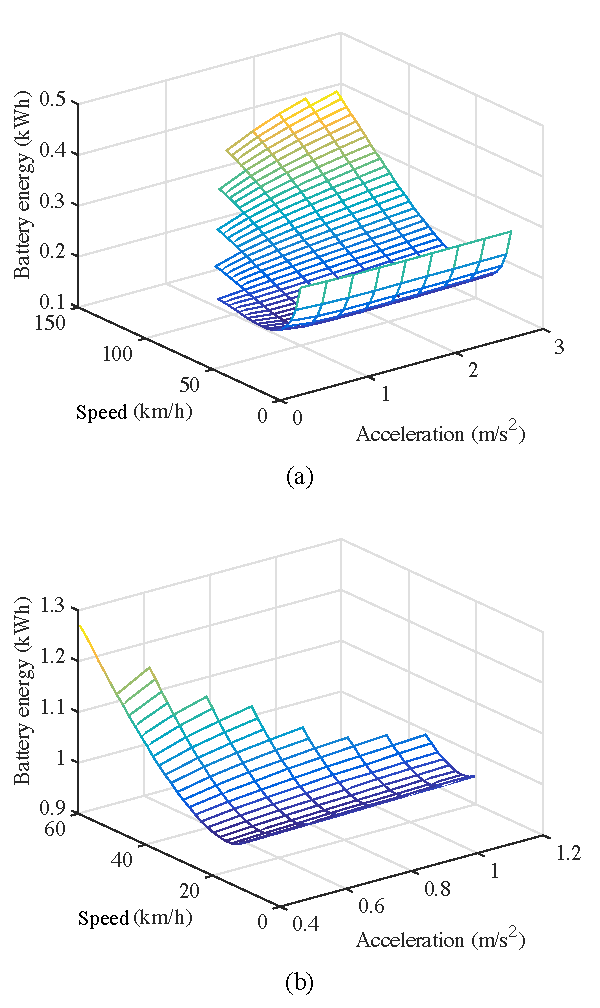
\includegraphics[width=0.9\hsize]{Figures/DSE.pdf}
\caption{Design space exploration of (a) Tesla Model S and (b) BYD K9.}
\label{fig:DSE}
\end{figure} 


We demonstrate how the cruising speed, acceleration and deceleration affect BEV energy consumption. We perform a design space exploration (DSE) for all feasible BEV speeds and the acceleration pairs. The results of DSE on an BEV sedan (Model S) and bus (K9) are shown in Fig.~\ref{fig:DSE}. 
We obtain the minimum-energy speed and the initial and final acceleration for a given driving distance. 
The point at the minimum-energy consumption per distance (Wh/km) represents the least-energy-constant-speed driving. The energy consumption by the cruising speed and acceleration pairs also completely changes by the BEV type. 
Each BEV type has different curb weight, motor specification, body shape, and tire, which affect energy consumption by acceleration and cruising speed, and, therefore, each BEV type has different least-energy-constant-speed driving.

\subsection{Problem formulation} \label{subsec:problem}

\begin{figure}	%Fig. 2
\centering
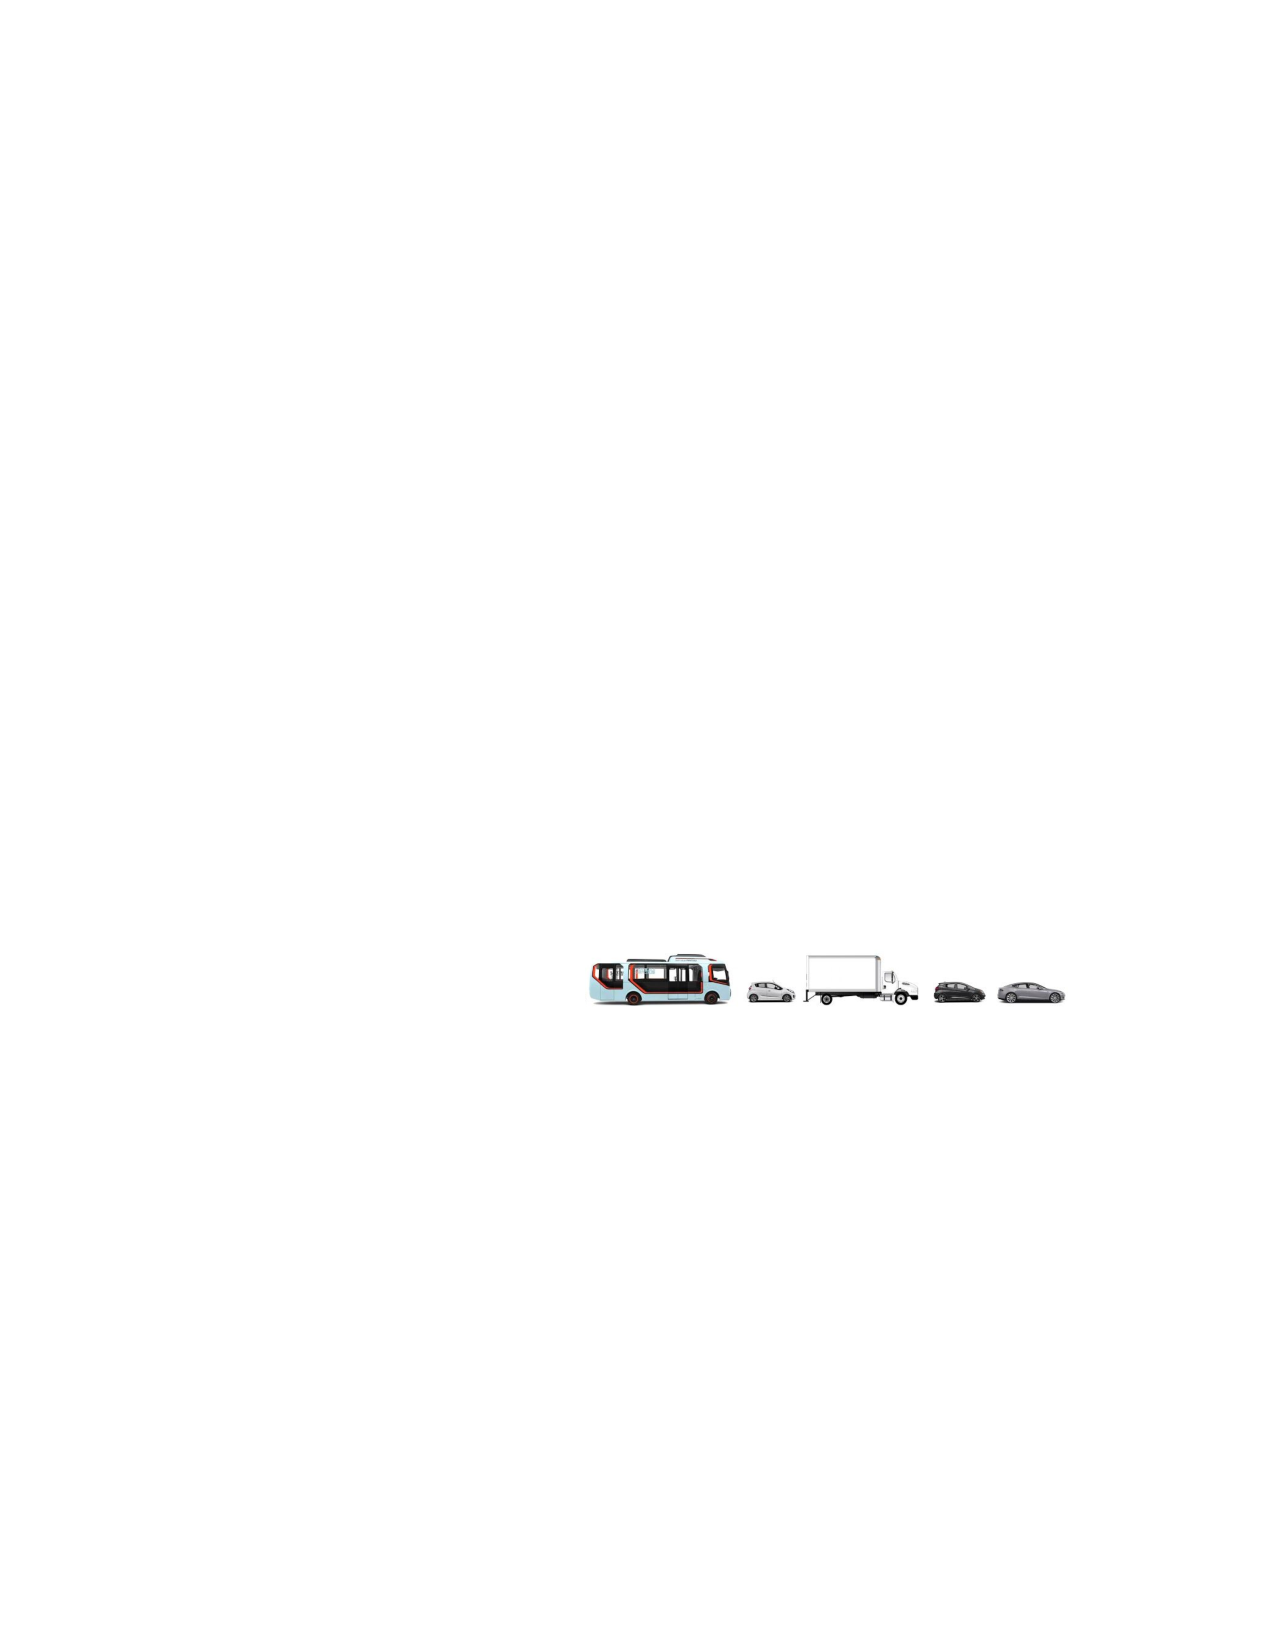
\includegraphics[width=1.0\hsize]{Figures/Example.pdf}
\caption{An example of a formation driving of heterogeneous BEVs on a single lane.}
\label{fig:example}
\end{figure} 

A set of formation BEVs on the same lane. $N$ BEVs, and a BEV $EV_i$ has a power models defined by~\eqref{eq:dynamics_model}, \eqref{eq:EV_specific_model}, \eqref{eq:regen_model}, and related coefficients in Table~\ref{table:Coeff_EVs}.
No interference is assumed for the formation, i.e., no other vehicles, no pedestrians, etc.
The formation driving consists of three stages: a constant acceleration, a constant-speed cruising and a constant deceleration.
A segment of the formation driving is from a signal to a signal, a stop sign to a stop sign, and so forth.
Use of a V2V communication, BEVs in the same formation can share their vehicle information, i.e., power model coefficients.
Each BEV weight is defined by the curb weight and the payload: passengers and cargos. The curb weight is known a priori, and the payload is measured by the sensor. 

Baseline is defined as following:
\begin{enumerate}
\item Ideal driving: each vehicle has its own minimum-energy acceleration, cruising speed and deceleration. 
It is permitted to pass a preceding vehicle.
\item Bounded driving: each vehicle has its own minimum-energy acceleration, cruising speed and deceleration guideline. If the acceleration or cruising speed of the preceding vehicle is slower than that of the following vehicle, the acceleration or cruising speed of the following vehicle is bounded to that of the preceding vehicle.
\end{enumerate}

%Problem
For a given formation, a set of BEV and their order, minimize the total energy consumption.
The formation acceleration, cruising speed and deceleration is defined by the recommended reference. Each BEV may not follow the formation driving reference as long as it does not interfere other BEV formation driving. For example, the first BEV may be driven faster than the formation cruising speed as long as it exhibits a smaller energy consumption.
Calculate the least-energy acceleration, cruising speed and deceleration.

%%%%%%%%%%%%%%%%%%%%%%%%%%%%%
\section{Experimental Results}\label{sec:exp}
%%%%%%%%%%%%%%%%%%%%%%%%%%%%%

\subsection{Driving Comparison by Vehicle Type}

\begin{table} 	%Table 2.
\centering
\small
\caption{List of BEVs and their vehicle type.}
\label{table:list_EVs}
\begin{tabular}{|c|c|c|c|c|c|} \hline
Index	&Vehicle	&Type		&Index	&Vehicle	&Type 	\\ \hline
1		&Bolt	&hatchback	&4		&K9		&bus			\\ \hline	
2		&Spark	&hatchback	&5		&Roadster&convertible 	\\ \hline
3		&Model S	&sedan	\\ \cline{1-3}
\end{tabular}
\end{table}

\begin{figure}	%Fig. 3
\centering
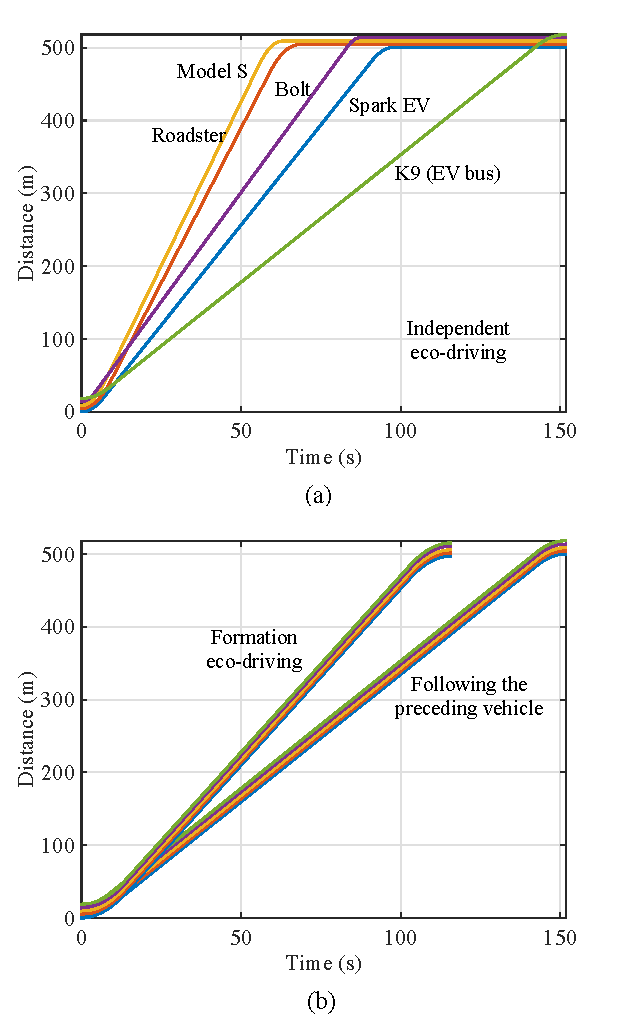
\includegraphics[width=1.0\hsize]{Figures/Heterogeneous_driving.pdf}
\caption{Heterogeneous BEV driving by (a) passing a preceding vehicle is permitted, and (b) passing is not permitted.}
\label{fig:hetero_driving}
\end{figure} 

We assume an example driving of five BEVs in Table~\ref{table:list_EVs}. A formation is Spark (last) - Roadster - Model S - Bolt - K9 (lead.)
The distance of this example is 500 m, and each BEV has its own minimum-energy acceleration and cruising speed. 
Fig.~\ref{fig:hetero_driving}(a) shows the ideal driving of the five BEVs over time if it is permitted to pass a preceding vehicle.  
Each BEV arrives at the endpoint in different time because they drive with different acceleration and cruising speed.
K9 starts at the forefront on the starting point. But, this BEV arrives at the endpoint the latest because the minimum-energy cruising speed of K9 is the slowest among all BEVs.
Fig.~\ref{fig:hetero_driving}(b) shows the drivings of the five BEVs if it is not permitted to pass a preceding vehicle. 

In the case of conventional bounded driving, the acceleration and cruising speed are bounded to those of the preceding vehicle. Therefore, acceleration and cruising speed of all BEVs are bounded to those of K9 in this example. Total energy consumption of the five BEVs is as 109.7\% of the energy consumption of the ideal driving.
On the other hands, if they drive with the proposed driving guideline mentioned in Section~\ref{subsec:problem}, it consume only 104.0\% of energy consumption of the ideal driving.
This means that increasing the acceleration and cruising speed of the bus is more efficient for all BEVs in the given formation.

\subsection{Driving Case Study}

\begin{table} 	%Table 3.
\centering
\small
\caption{List of heterogeneous driving formations.}
\label{table:list_formation}
\begin{tabular}{|c|c|} \hline
No.	&EV formation from last to lead	\\ \hline
1	&3 2 3 5 3 5 1 5 3 4	\\ \hline
2	&3 2 3 5 3 5 3 4 5 1	\\ \hline
3	&3 5 3 4 5 3 5 3 2 1	\\ \hline
4	&4 3 2 3 5 3 5 1 5 3	\\ \hline
\end{tabular}
\end{table}

\begin{figure}	%Fig. 4
\centering
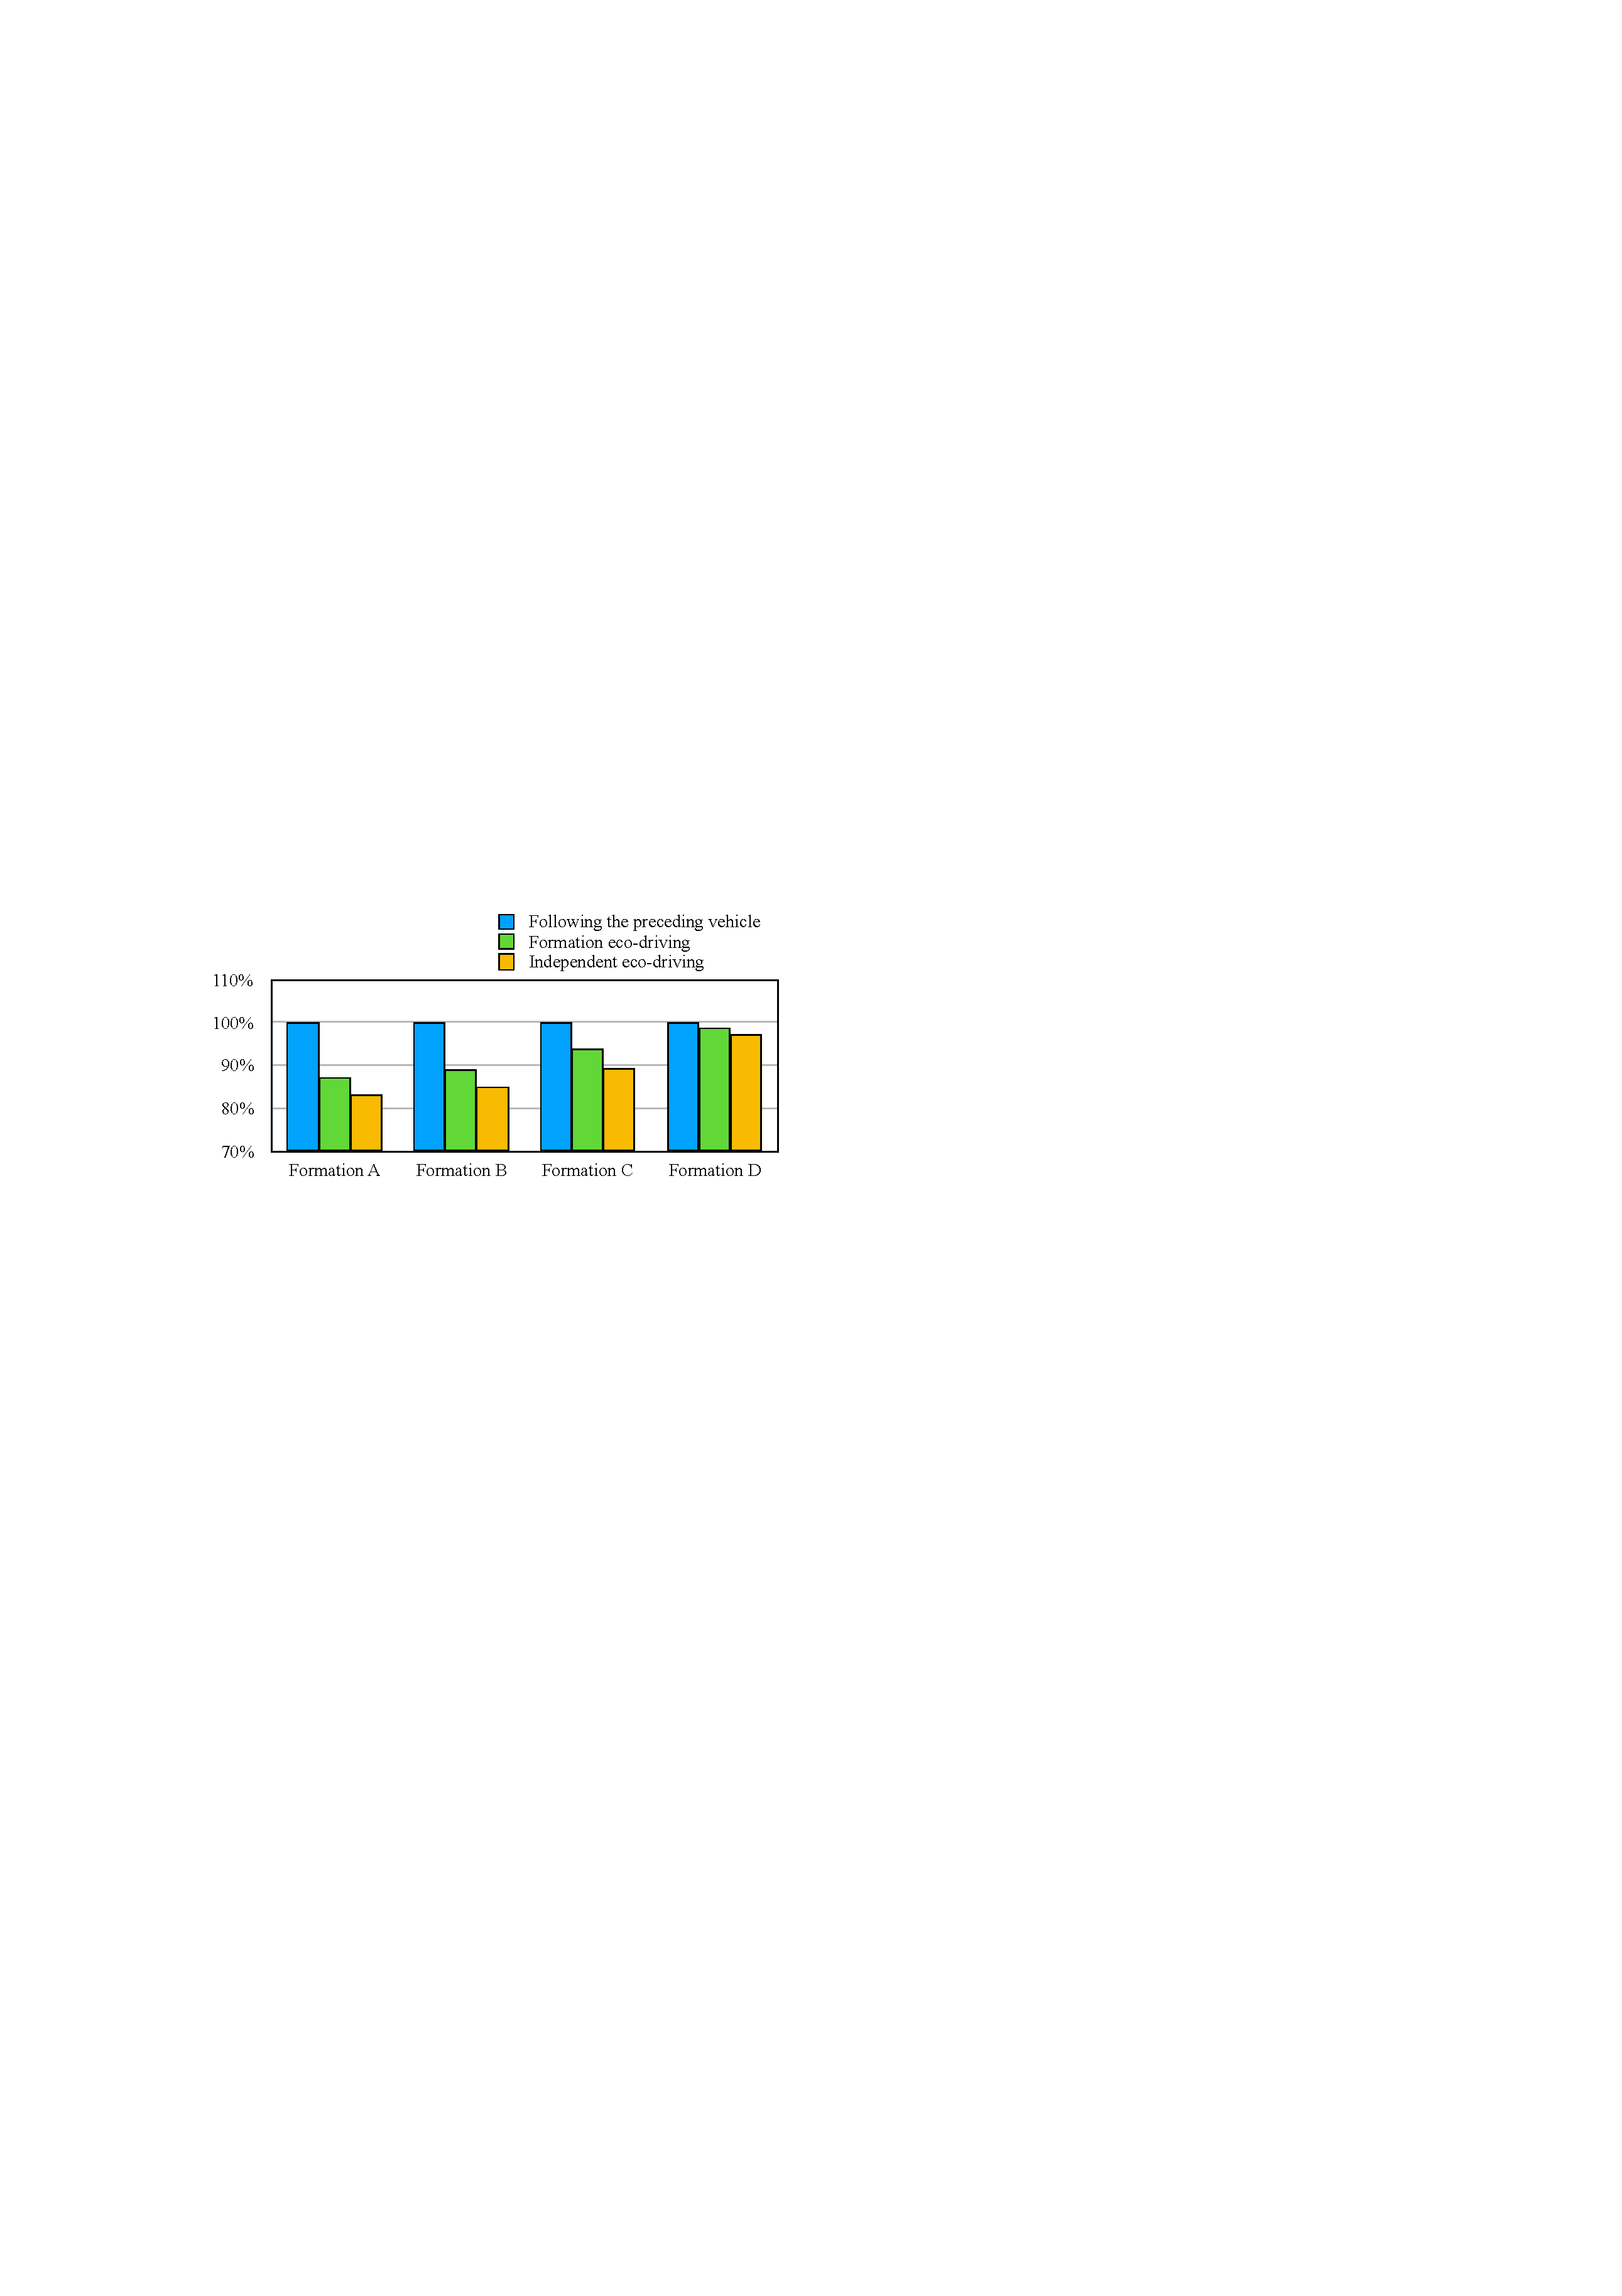
\includegraphics[width=1.0\hsize]{Figures/Bar_graph.pdf}
\caption{Heterogeneous driving results by BEV formations.}
\label{fig:bar_graph}
\end{figure} 

We assume a case study of heterogeneous BEV driving with 10 BEVs. Table~\ref{table:list_formation} shows the formations of 10 BEVs. 
Fig.~\ref{fig:bar_graph} shows the comparisons of the energy consumption of 10 BEVs for the driving. Blue bars indicate the energy consumption by the bounded driving, in which the vehicle driving is bounded by the preceding vehicle. Blue bars show 100\% energy consumption in this figure. Green bars indicate the energy consumption by the proposed group driving method, and orange bars indicate ideal driving, which is possible to pass a preceding BEV.
The energy gain by the proposed group driving compared with the bounded driving is from 1.41\% to 12.81\%. 

In case of formation 1, the bus is lead, and it is very common when group driving is limited by a bus ahead. In this formation, drivings of all BEVs are bounded to the least-energy-constant-speed driving of the bus. The gain by the proposed group driving is 12.81\% compared with the bounded driving.
In case of formation 4, the least-energy-constant-speeds of two leading BEVs (hatchback and convertible) are faster than a recommended reference, and that of the last BEV (bus) is slower than the reference. Therefore, these three BEVs drive their own optimal, and only seven BEVs follow the reference as shown in Fig.~\ref{fig:driving_comp}.

\begin{figure}	%Fig. 5
\centering
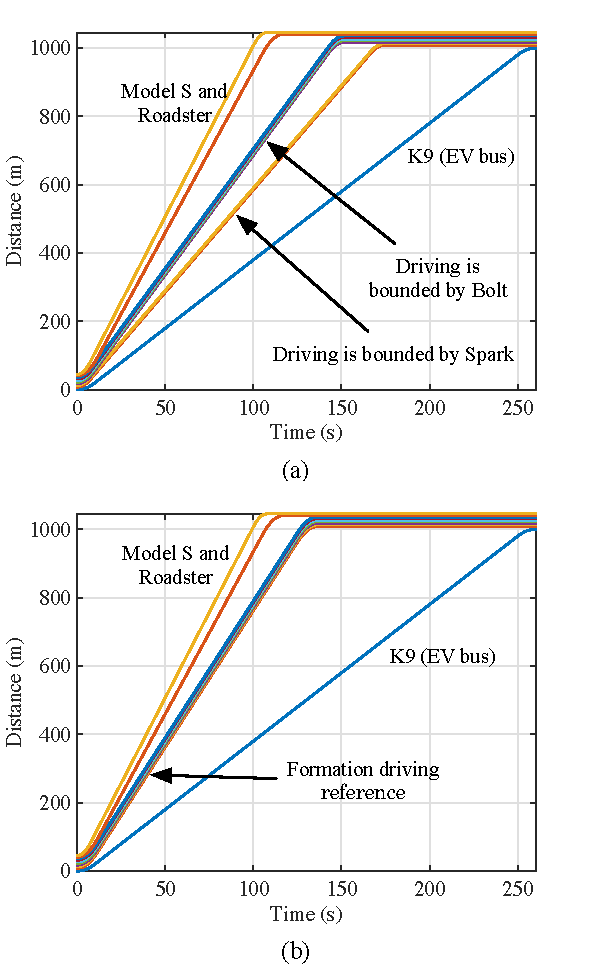
\includegraphics[width=1.0\hsize]{Figures/Driving_comparison.pdf}
\caption{Heterogeneous BEV driving result of  (a) bounded driving and (b) proposed driving in case of formation 4.}
\label{fig:driving_comp}
\end{figure} 


%%%%%%%%%%%%%%%%%%%%%%%%%%%%%%
\section{Conclusions}
%%%%%%%%%%%%%%%%%%%%%%%%%%%%%%

%%%%%%%%%%%%%%%%%%%%%%%%%%%%%%%%%%%%%%%%%%
%\section*{Acknowledgment}
%%%%%%%%%%%%%%%%%%%%%%%%%%%%%%%%%%%%%%%%%%
%This work was supported by the National Research Foundation of Korea(NRF) grant funded by the Korea government(MSIP) (No.2015R1A2A1A09005694)

\bibliographystyle{ieeetr}
\bibliography{EV}

% that's all folks
\end{document}
